\documentclass{article}
\usepackage[left=1.5cm, right=1.5cm, top=1.5cm, bottom=2cm]{geometry}
\usepackage[utf8]{inputenc}
\usepackage{amsmath,amsthm,stmaryrd,amssymb,bbm,amsfonts,amstext,graphicx,multicol,array}
\usepackage{subfigure}
\usepackage{xcolor}
\usepackage{enumitem}
\usepackage{indentfirst}
\usepackage{caption}
\usepackage{pdfpages}
\usepackage[numbers]{natbib} % Use natbib with numerical citations
\usepackage{hyperref}
\usepackage{float}
\usepackage{booktabs}
\usepackage{graphics, graphicx}
\usepackage{booktabs}
\usepackage{adjustbox}

\hypersetup{
    colorlinks=true,
    linkcolor=blue,
    urlcolor=blue,
    citecolor=blue
}

\setlength{\parindent}{2em}
\setlength{\parskip}{1em}
\renewcommand{\baselinestretch}{1.5}

\title{ECON2390 Fall 2024\\Applied Econometrics\\Problem Set 2}
\author{Adrien Foutelet}
\date{October 2024}

\begin{document}

\maketitle

\section{Regression Discontinuity Design}

%%%%%%%%%%%%%%%%%%%%%%%%%%%%%%%%%%%%%%%%%%%%%%%%%%%%%%%%%%%%%%%
\subsection{}

We run OLS to estimate the following model:
\[Y_m = \beta_0 + \beta_1 \text{PANwin}_m + \epsilon_m\]

We get the following estimates (see table \ref{tab:model1}).

\begin{table}[htbp]\centering
\def\sym#1{\ifmmode^{#1}\else\(^{#1}\)\fi}
\caption{Simple OLS regression model\label{tab:model1}}
\begin{tabular}{l*{1}{c}}
\toprule
                    &\multicolumn{1}{c}{Y}\\
\midrule
(mean) PANwin       &       0.904         \\
                    &      (0.06)         \\
\addlinespace
Constant            &       43.63\sym{***}\\
                    &      (4.58)         \\
\midrule
Observations        &         152         \\
\bottomrule
\multicolumn{2}{l}{\footnotesize \textit{t} statistics in parentheses}\\
\multicolumn{2}{l}{\footnotesize \sym{*} \(p<0.05\), \sym{**} \(p<0.01\), \sym{***} \(p<0.001\)}\\
\end{tabular}
\end{table}


The positive correlation between variables Y and PANwin that the coefficient suggests does not appear to be significant.

We may be facing endogeneity:
\begin{itemize}
    \item It is where the homicide rate is high and the drug trafficking organisations have strong presence that the party promoting radical anti drug policies is elected (reverse causality);
    \item PAN may have prioritized campaigning in dangerous areas where their agenda gave them the best chances to wind (selection);
    \item In some places, the local culture may be more martial, making PAN most popular, a cultural trait that may result from weaker state capacity, which is suitable for criminal organisations to thrive (omitted variable bias).
\end{itemize}
We need to isolate exogenous variations in PANwin to infer causal results.

For these reasons, \(\beta_1\) should be positively biased and \(\beta_0\) should be negatively biased.

%%%%%%%%%%%%%%%%%%%%%%%%%%%%%%%%%%%%%%%%%%%%%%%%%%%%%%%%%%%%%%%
\subsection{}

The key assumption necessary for the fuzzy regression discontinuity design to be valid in Dell's analysis is:
\begin{itemize}
    \item The continuity assumption: there is continuity of the potential outcomes at the cutoff.
\end{itemize}

In practice, it is necessary that:
\begin{itemize}   
    \item All relevant factors besides treatment vary smoothly at the threshold between a PAN victory and loss.
    \item There is absence of selective sorting around the PAN win-loss threshold.
\end{itemize}


%%%%%%%%%%%%%%%%%%%%%%%%%%%%%%%%%%%%%%%%%%%%%%%%%%%%%%%%%%%%%%%

\subsection{}

Investigating whether the regression discontinuity design shows evidence of manipulation, we do a McCrary test for the following null hypothesis:

\[H_0: \text{ "The density of the running variable is continuous at the cutoff"}\]

We get the following results (see table \ref{tab:McCrary}):
\begin{table}[htbp]\centering
\caption{McCrary density test\label{tab:McCrary}}
\begin{tabular}{l*{1}{c}}
\hline\hline
            &\multicolumn{1}{c}{margin\_victory}\\
\hline
\hline
LogDensityRatio&     -0.0763\\
StdError    &       24.19\\
PValue      &       0.939\\
Bandwidth\_left&      0.0135\\
Bandwidth\_right&      0.0157\\
\hline\hline
\end{tabular}
\end{table}


Our high p-value implies that we fail to reject the null hypothesis, meaning that we find no evidene of significant difference in the density of the running variable on either side of the cutoff.

We get the following plot of the estimated density of the running variable on both sides of the cutoff (see figure \ref{fig:McCrary}). No visual discontinuity can be found in the density at the cutoff: the density is smooth. 

\begin{figure}[H]
    \centering
    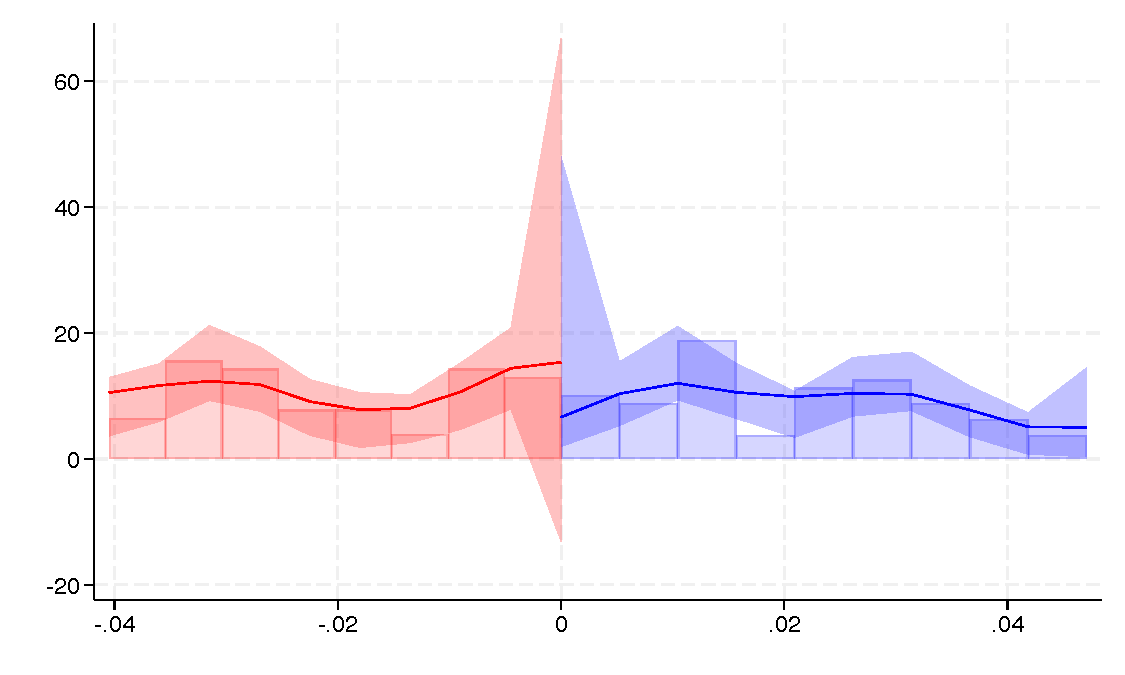
\includegraphics[width=\textwidth]{../outputs/mccrary_plot.pdf}
    \caption{McCrary test result plot}
    \label{fig:McCrary}
\end{figure}

It makes sense because it is very unlikely that the voters, in a general election, know the results in advance and change their behavior accordingly to get a precise margin of victory close to the cutoff.

%%%%%%%%%%%%%%%%%%%%%%%%%%%%%%%%%%%%%%%%%%%%%%%%%%%%%%%%%%%%%%%

\subsection{}

\begin{figure}[H]
    \centering
    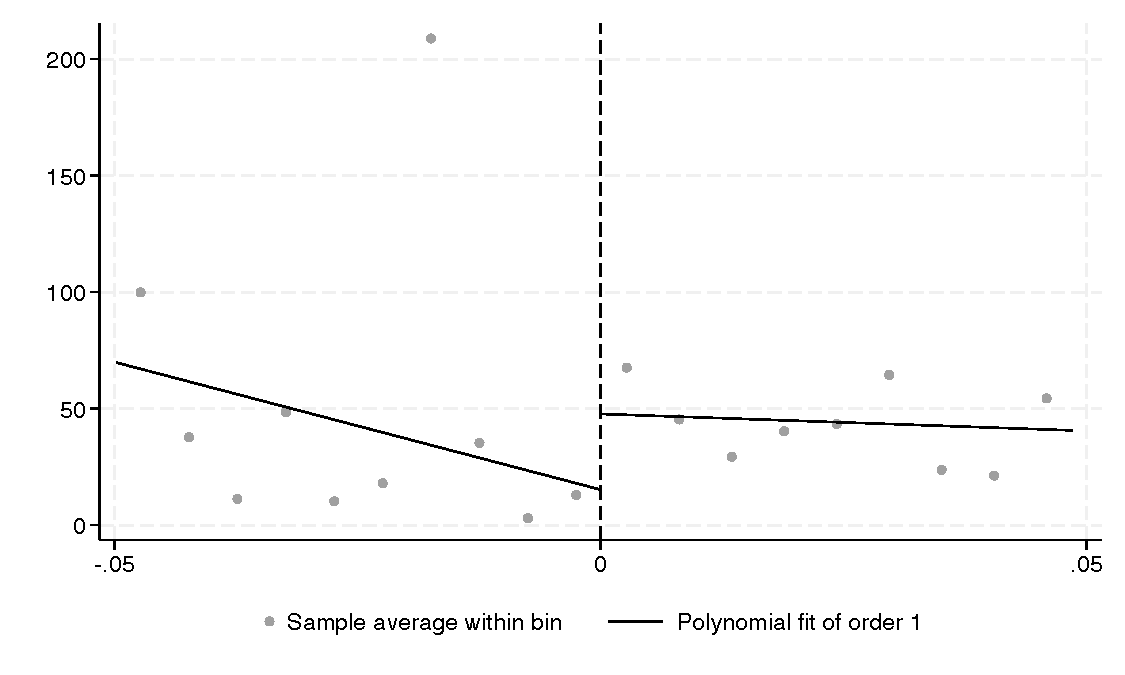
\includegraphics[scale=0.5]{../outputs/binned_scatter_esmv_linear_plot.pdf}
    \caption{Binned scatter plot of PAN victory margin and homicide rate (number of bins selected via mimicking variance evenly-spaced method using spacings estimators, linear specification)}
    \label{fig:binned_scatter_esmv_linear}
\end{figure}

\begin{figure}[H]
    \centering
    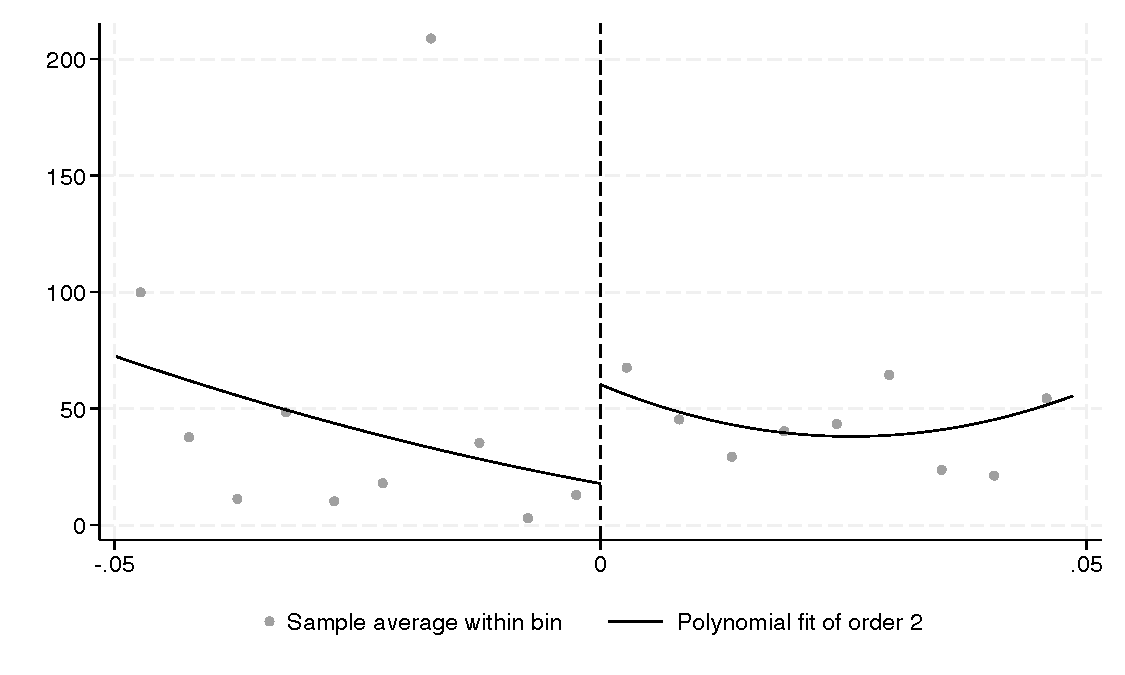
\includegraphics[scale=0.5]{../outputs/binned_scatter_esmv_quadratic_plot.pdf}
    \caption{Binned scatter plot of PAN victory margin and homicide rate (number of bins selected via mimicking variance evenly-spaced method using spacings estimators, quadratic specification)}
    \label{fig:binned_scatter_esmv_quadratic}
\end{figure}

\begin{figure}[H]
    \centering
    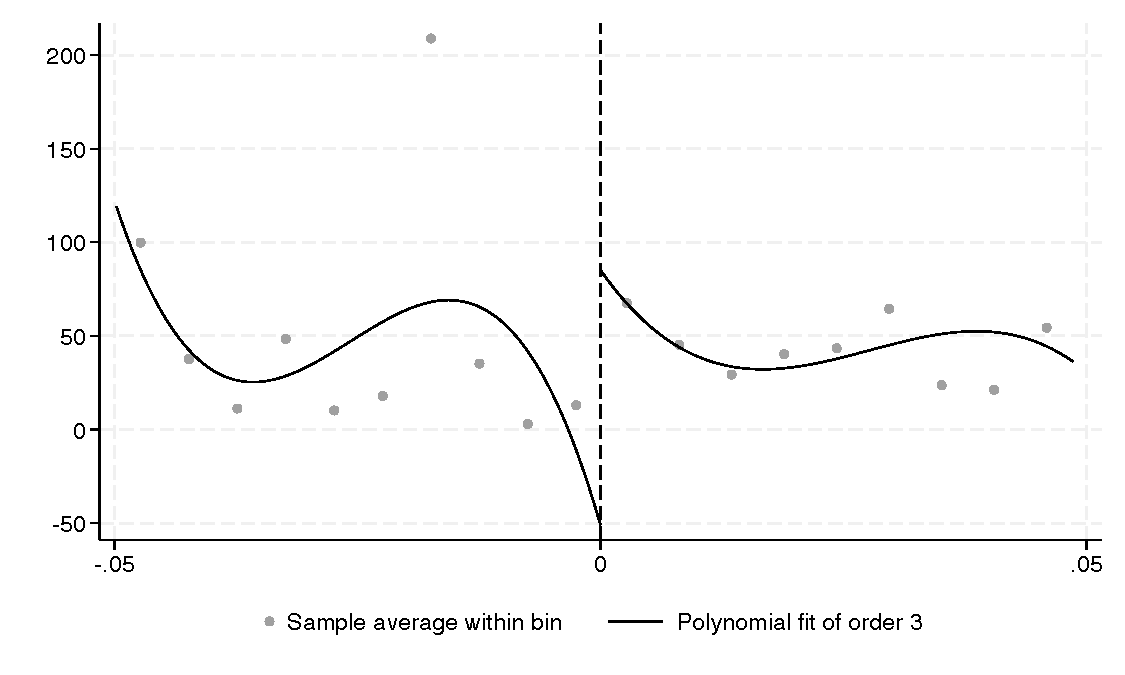
\includegraphics[scale=0.5]{../outputs/binned_scatter_esmv_cubic_plot.pdf}
    \caption{Binned scatter plot of PAN victory margin and homicide rate (number of bins selected via mimicking variance evenly-spaced method using spacings estimators, cubic specification)}
    \label{fig:binned_scatter_esmv_cubic}
\end{figure}

\begin{figure}[H]
    \centering
    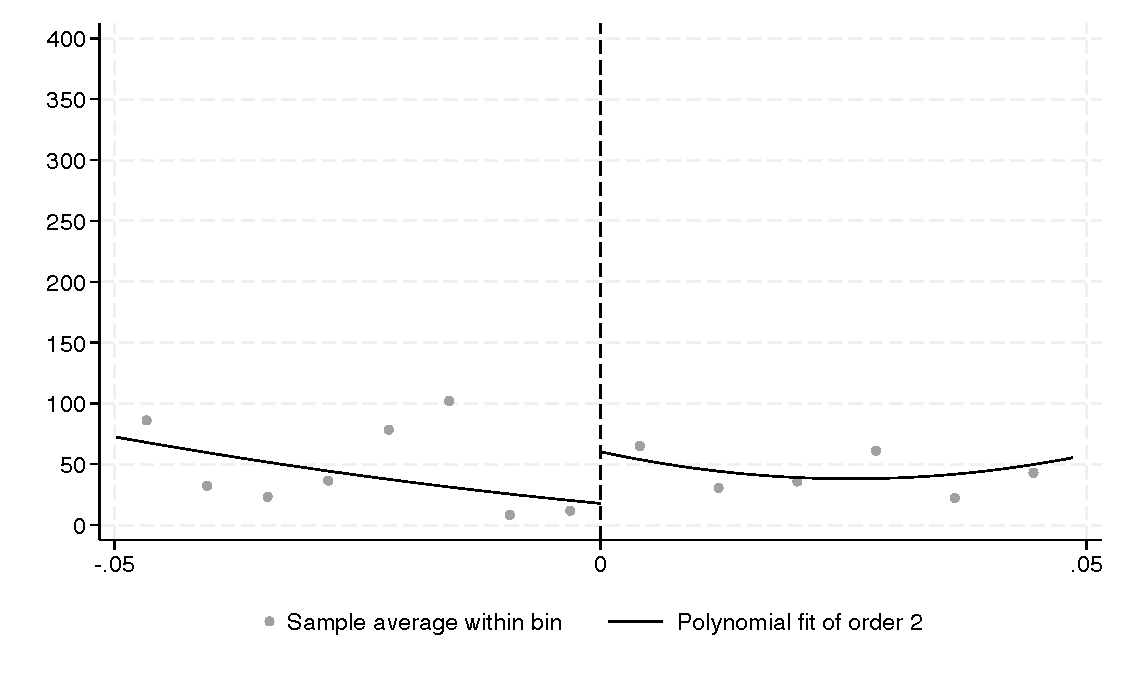
\includegraphics[scale=0.5]{../outputs/binned_scatter_es_cubic_plot.pdf}
    \caption{Binned scatter plot of PAN victory margin and homicide rate (number of bins selected via IMSE-optimal evenly-spaced method using spacings estimators, cubic specification)}
    \label{fig:binned_scatter_es_cubic}
\end{figure}

\begin{figure}[H]
    \centering
    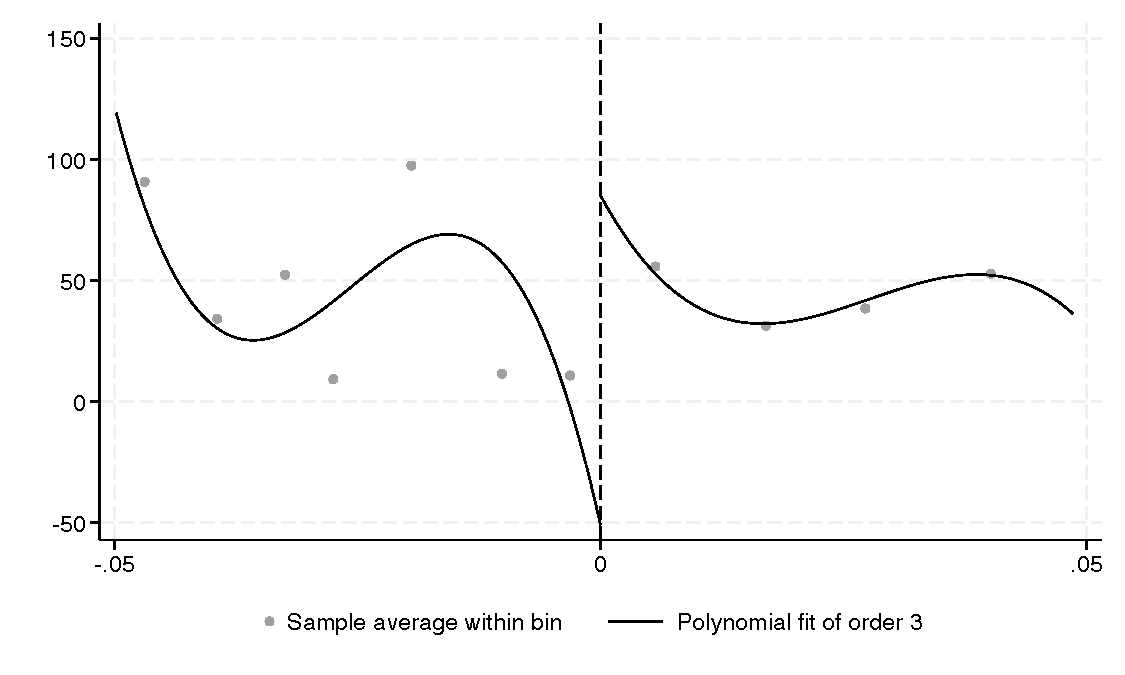
\includegraphics[scale=0.5]{../outputs/binned_scatter_qs_cubic_plot.pdf}
    \caption{Binned scatter plot of PAN victory margin and homicide rate (number of bins selected via IMSE-optimal quantile-spaced method using spacings estimators, cubic specification)}
    \label{fig:binned_scatter_qs_cubic}
\end{figure}

\begin{figure}[H]
    \centering
    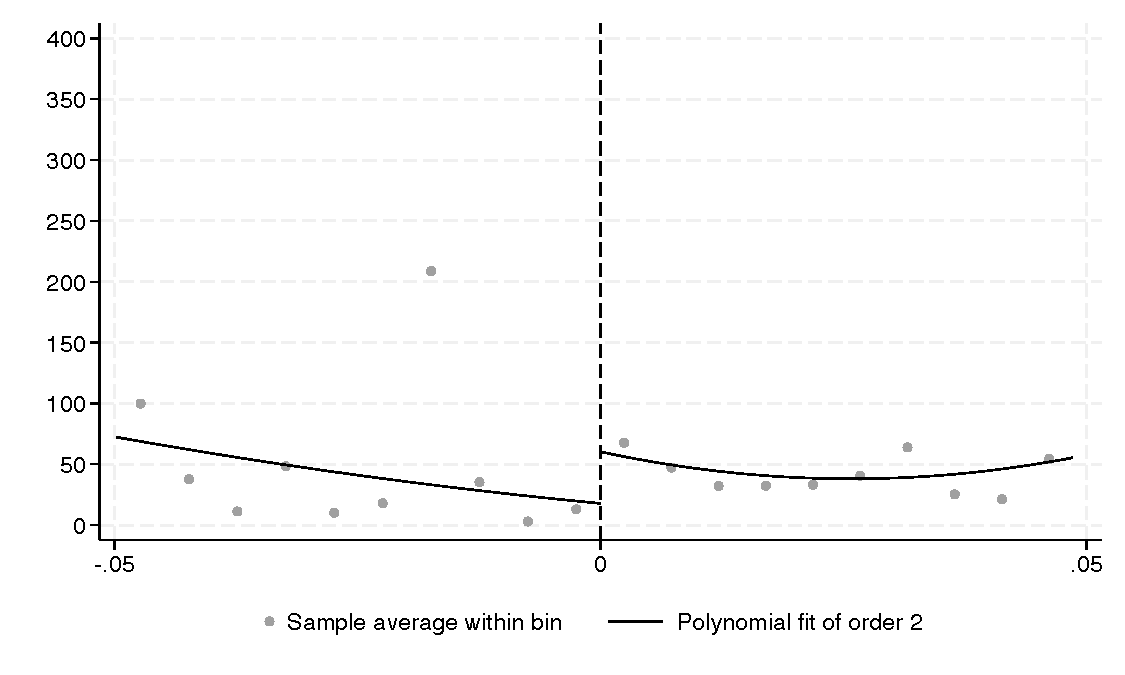
\includegraphics[scale=0.5]{../outputs/binned_scatter_10bins_cubic_plot.pdf}
    \caption{Binned scatter plot of PAN victory margin and homicide rate (number of bins bormatively set at 10, cubic specification)}
    \label{fig:binned_scatter_10bins_cubic}
\end{figure}

\begin{figure}[H]
    \centering
    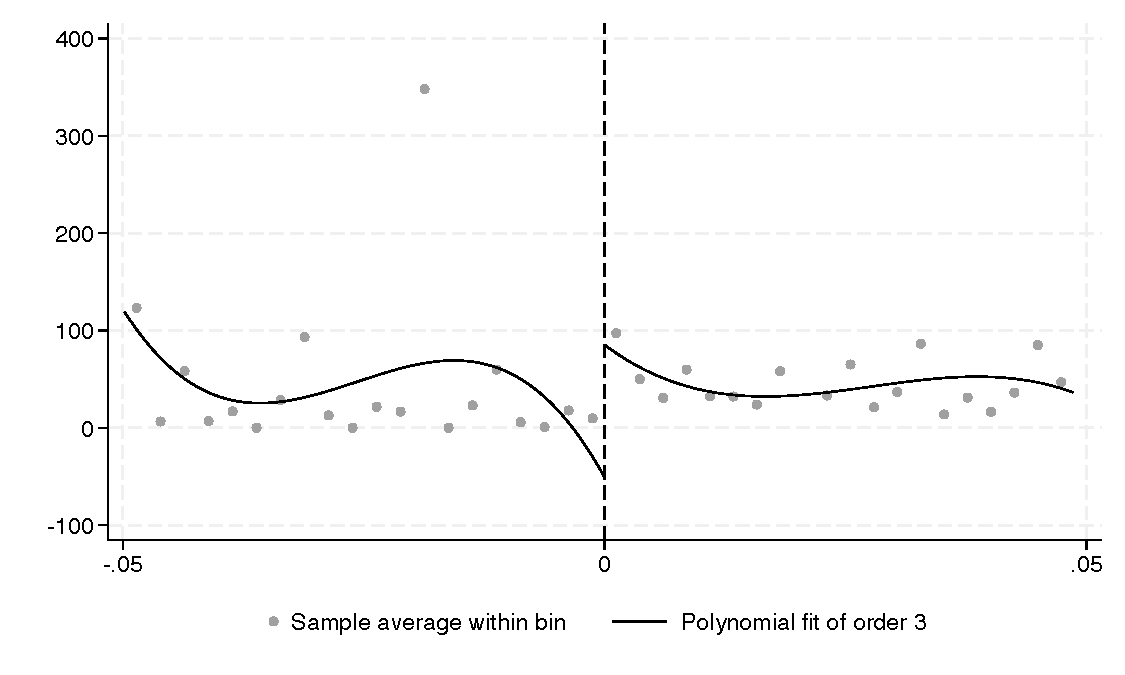
\includegraphics[scale=0.5]{../outputs/binned_scatter_20bins_cubic_plot.pdf}
    \caption{Binned scatter plot of PAN victory margin and homicide rate (number of bins bormatively set at 20, cubic specification)}
    \label{fig:binned_scatter_20bins_cubic}
\end{figure}

The discontinuity at the cutoff is robust to the three polynomial specifications (see figures \ref{fig:binned_scatter_esmv_linear}, \ref{fig:binned_scatter_esmv_quadratic}, \ref{fig:binned_scatter_esmv_cubic}, \ref{fig:binned_scatter_es_cubic}, \ref{fig:binned_scatter_qs_cubic}, \ref{fig:binned_scatter_10bins_cubic}, \ref{fig:binned_scatter_20bins_cubic}). However, the degree three specification seems to suffer from overfitting: there is no justification explaining the variations clost to the cutoff and the large discontinuity seems fabricated.

The discontinuity at the cutoff is robust to the five procedures for bin number selection, with no major difference in the size of the cutoff.

%%%%%%%%%%%%%%%%%%%%%%%%%%%%%%%%%%%%%%%%%%%%%%%%%%%%%%%%%%%%%%%

\subsection{}

We get the following estimates (see table \ref{tab:model2}).

\begin{table}[htbp]\centering
\def\sym#1{\ifmmode^{#1}\else\(^{#1}\)\fi}
\caption{Non-parametric and parametric RDD models\label{tab:model2}}
\begin{tabular}{l*{4}{c}}
\toprule
                    &\multicolumn{1}{c}{Non-para tri lin}&\multicolumn{1}{c}{Non-para tri quad}&\multicolumn{1}{c}{Para lin}&\multicolumn{1}{c}{Para quad}\\
\midrule
RD\_Estimate         &       80.25\sym{*}  &       93.93         &                     &                     \\
                    &      (2.25)         &      (1.92)         &                     &                     \\
\addlinespace
(mean) spread       &                     &                     &       979.5         &      2697.6         \\
                    &                     &                     &      (0.36)         &      (0.39)         \\
\addlinespace
(mean) PANwin       &                     &                     &       69.99\sym{**} &       81.79\sym{*}  \\
                    &                     &                     &      (2.91)         &      (2.57)         \\
\addlinespace
(mean) PANwin=1 $\times$ (mean) spread&                     &                     &     -5770.9         &    -12951.7         \\
                    &                     &                     &     (-1.50)         &     (-1.31)         \\
\addlinespace
(mean) spread squared&                     &                     &                     &    260133.0         \\
                    &                     &                     &                     &      (0.54)         \\
\addlinespace
(mean) PANwin=1 $\times$ (mean) spread squared&                     &                     &                     &    138247.6         \\
                    &                     &                     &                     &      (0.21)         \\
\addlinespace
Constant            &                     &                     &       12.95         &       14.37         \\
                    &                     &                     &      (0.78)         &      (0.66)         \\
\midrule
Observations        &         152         &         152         &          38         &          54         \\
\bottomrule
\multicolumn{5}{l}{\footnotesize \textit{t} statistics in parentheses}\\
\multicolumn{5}{l}{\footnotesize \sym{*} \(p<0.05\), \sym{**} \(p<0.01\), \sym{***} \(p<0.001\)}\\
\end{tabular}
\end{table}


We get significant RDD estimates for the non-parametric-trianguler-kernel-degree 1 case, for the parametric-degree 1 case, and for the parametric-degree 2 case. Hence the significance seems to be better overall for the parametric models in our case.

The magnitudes of the estimates of the parametric and non-parametric estimates are close to one another.

The magnitudes are greater than that of our rdplot discontinuities. That is due to the fact that the bandwidth used by default with rdplot differs from the optimal bandwidth selected by rdrobust. For example, if we choose the same bandwidth with rdplot for the parametric-linear case, we get a consistent discontinuity (see figure \ref{fig:binned_scatter_esmv_linear_corrected}).

\begin{figure}[H]
    \centering
    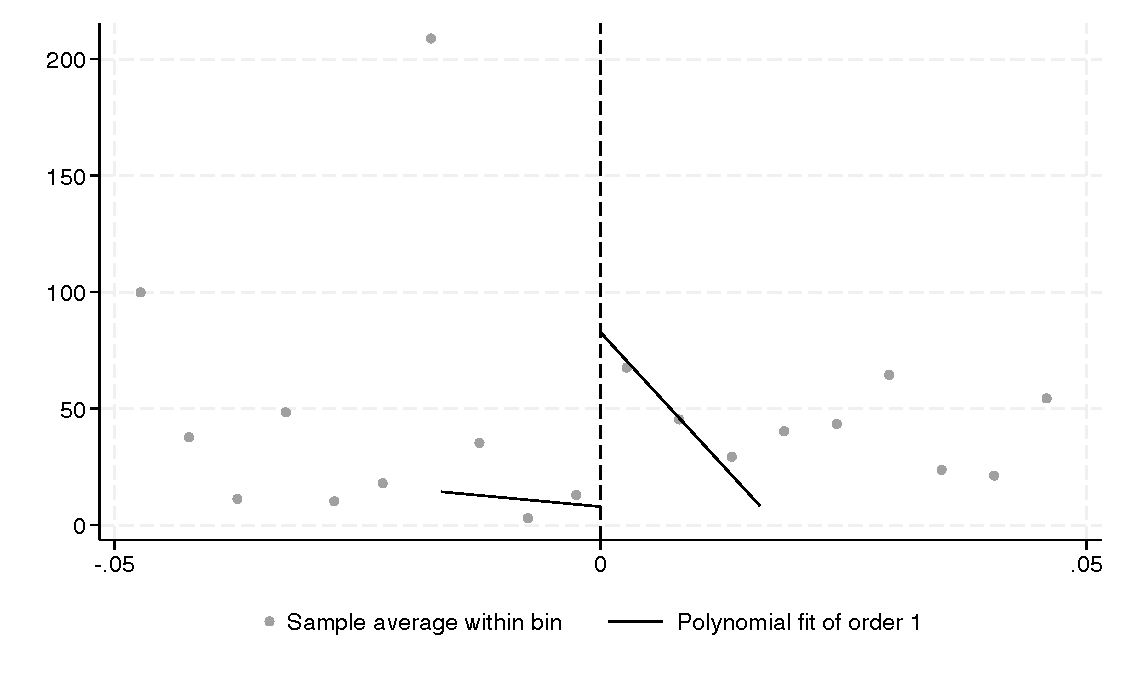
\includegraphics[scale=0.5]{../outputs/binned_scatter_esmv_linear_plot_corrected.pdf}
    \caption{Binned scatter plot of PAN victory margin and homicide rate matching with a bandwidth matching the standard rdrobust one (number of bins selected via mimicking variance evenly-spaced method using spacings estimators, linear specification)}
    \label{fig:binned_scatter_esmv_linear_corrected}
\end{figure}

The parametric-specific RDD assumptions:
\begin{itemize}
    \item A functional form is assumed for \(E(Y \mid X)\), allowing for different parameters on either side of the cutoff.
    \item All observations are used regardless of their distance from the cutoff (the functional form holds globally).
\end{itemize}

The non-parametric-specific RDD assumptions:
\begin{itemize}
    \item Local continuity of the potential outcomes i.e., potential outcomes are assumed to be smooth within a small neighborhood of the cutoff and the estimation focuses only on this local region,
    \item A bandwidth must be chosen around the cutoff to balance:
    \begin{itemize}
        \item Bias from including too many observations far from the cutoff,
        \item Variance from using too few observations,
    \end{itemize}
    \item Observations are weighted based on their distance from the cutoff, typically giving more weight to those loser to it,
    \item The small sample nature of the local estimates calls for bias correction and robust variance estimation.
\end{itemize}

Parametric RDD is typically more precise (lower standard errors) but risks bias if the model is misspecified.
Non-parametric RDD sacrifices precision (higher standard errors) for robustness, making it better suited for estimating local effects near the cutoff with fewer assumptions. The choice depends on the situation:
\begin{itemize}
    \item If the functional form is likely well-specified: parametric methods give more precise estimates,
    \item If there is uncertainty about the functional form: non-parametric methods give more reliable but less precise results.
\end{itemize}

%%%%%%%%%%%%%%%%%%%%%%%%%%%%%%%%%%%%%%%%%%%%%%%%%%%%%%%%%%%%%%%

\subsection{}

We get the following estimates (see table \ref{tab:model2-robustness}) from the donut hole approach. This tests whether the observed treatment effect is driven by potential manipulation or discontinuities unrelated to the treatment itself. Indeed it reveals whether the units near the cutoff influence the results.

More precisely, if individuals manipulate their running variable, it is likely that those near the cutoff be different across treatment and control groups. Therefore, a similar treatment effect with and without the donut hole suggests no manipulation near the cutoff. Note what is interpreted as manipulation could also just be local anomalies around the cutoff, like outliers. The McCrary test invalidated these possibilities.

Here we do find a plumetting treatment effect after excluding 20\% of the optimal bandwidth on both sides. This apparent inconsistency with the results from the McCrary test is most proably explained by the fact that removing that many observations from the optimal bandwidth, especially the most weighted ones, is likely to reduce precision. We would need a critera to choose an appropriate donut hole size.

\begin{table}[htbp]\centering
\def\sym#1{\ifmmode^{#1}\else\(^{#1}\)\fi}
\caption{RDD model robustness\label{tab:model2-robustness}}
\begin{tabular}{l*{4}{c}}
\toprule
                    &\multicolumn{1}{c}{Para tri lin}&\multicolumn{1}{c}{Para tri lin 5\%}&\multicolumn{1}{c}{Para tri lin 10\%}&\multicolumn{1}{c}{Para tri lin 20\%}\\
\midrule
RD\_Estimate         &       80.25\sym{*}  &       80.25\sym{*}  &       98.36\sym{*}  &       48.95         \\
                    &      (2.25)         &      (2.25)         &      (2.14)         &      (1.00)         \\
\midrule
Observations        &         152         &         152         &         151         &         144         \\
\bottomrule
\multicolumn{5}{l}{\footnotesize \textit{t} statistics in parentheses}\\
\multicolumn{5}{l}{\footnotesize \sym{*} \(p<0.05\), \sym{**} \(p<0.01\), \sym{***} \(p<0.001\)}\\
\end{tabular}
\end{table}


\begin{figure}[H]
    \centering
    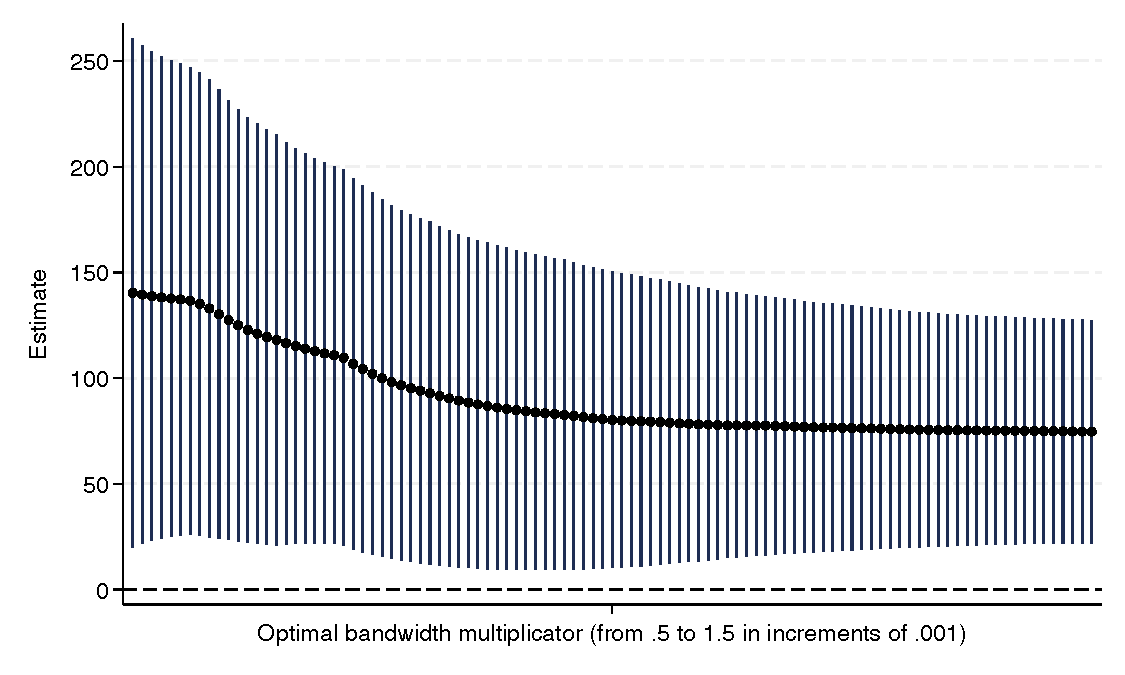
\includegraphics[scale=0.8]{../outputs/model2_robustness_plot.pdf}
    \caption{RDD model robustness}
    \label{fig:model2-robustness}
\end{figure}

Using a loop the re-estimate the model with bandwidths ranging from \(0.5\) to \(1.5\) times the optimal bandidth, we get the following graph (see figure \ref{fig:model2-robustness}). Recall that A bandwidth must be chosen around the cutoff to balance:
\begin{itemize}
    \item Bias from including too many observations far from the cutoff,
    \item Variance from using too few observations,
\end{itemize}
Here, as we increase the bandwidth, the confidence interval decreases, betraying shrinking variance. The magnitude of the estimates plateaus at the level of the one computed with the optimal bandwidth. This is likely to be specific to our model and dataset as it is not necessarily the case in the context of increasing bias. 

%%%%%%%%%%%%%%%%%%%%%%%%%%%%%%%%%%%%%%%%%%%%%%%%%%%%%%%%%%%%%%%

\subsection{}

John Marshall's concern about compensating differentials in Politician Characteristic Regression Discontinuity (PCRD) designs hints at the idea that these designs fail to isolate the pure effect of a politician's characteristic (e.g., gender, party affiliation) because other characteristics, known as compensating differentials, influence both the election outcome and downstream the effects.

For example, if voters are biased against women, female candidates in close elections may need to compensate by having higher levels of competence or qualifications than their male opponents. The characteristic of interest (e.g., gender) correlates with compensating differentials that offset its impact (e.g., competence).

This means that PCRD designs compare candidates who are not equivalent on other important traits, leading to biased estimates of the effect of the characteristic of interest, since the effect measured is a compound treatment effect of the characteristic of interest and the compensating differentials.

Marshall recommends to attempt to measure compensating differentials to bound or reinterpret the results.

Dell uses close elections to argue that PAN mayoral victories causally increase drug-related violence. The compensating differentials from winning PAN condidates may be:
\begin{itemize}
    \item Their strong-willed disruptive and uncompromising characters (prone to get drug dealers' backs up),
    \item Their expected lower level of corruption (prone to increase violence from the mobsters as the mayer would never compromise with them and cast a blind eye),
    \item Their stronger connections with federal authorities (prone to make anti crime policies even stronger locally and increase violence in retaliation),
    \item Their populist views rejecting sophisticated understanding of deviance (prone to make them both attractively radical and acting without tact).
\end{itemize} 
There would then be selection of these traits for the mayors in the treatment group.

\subsection{}

\begin{figure}
    \centering
    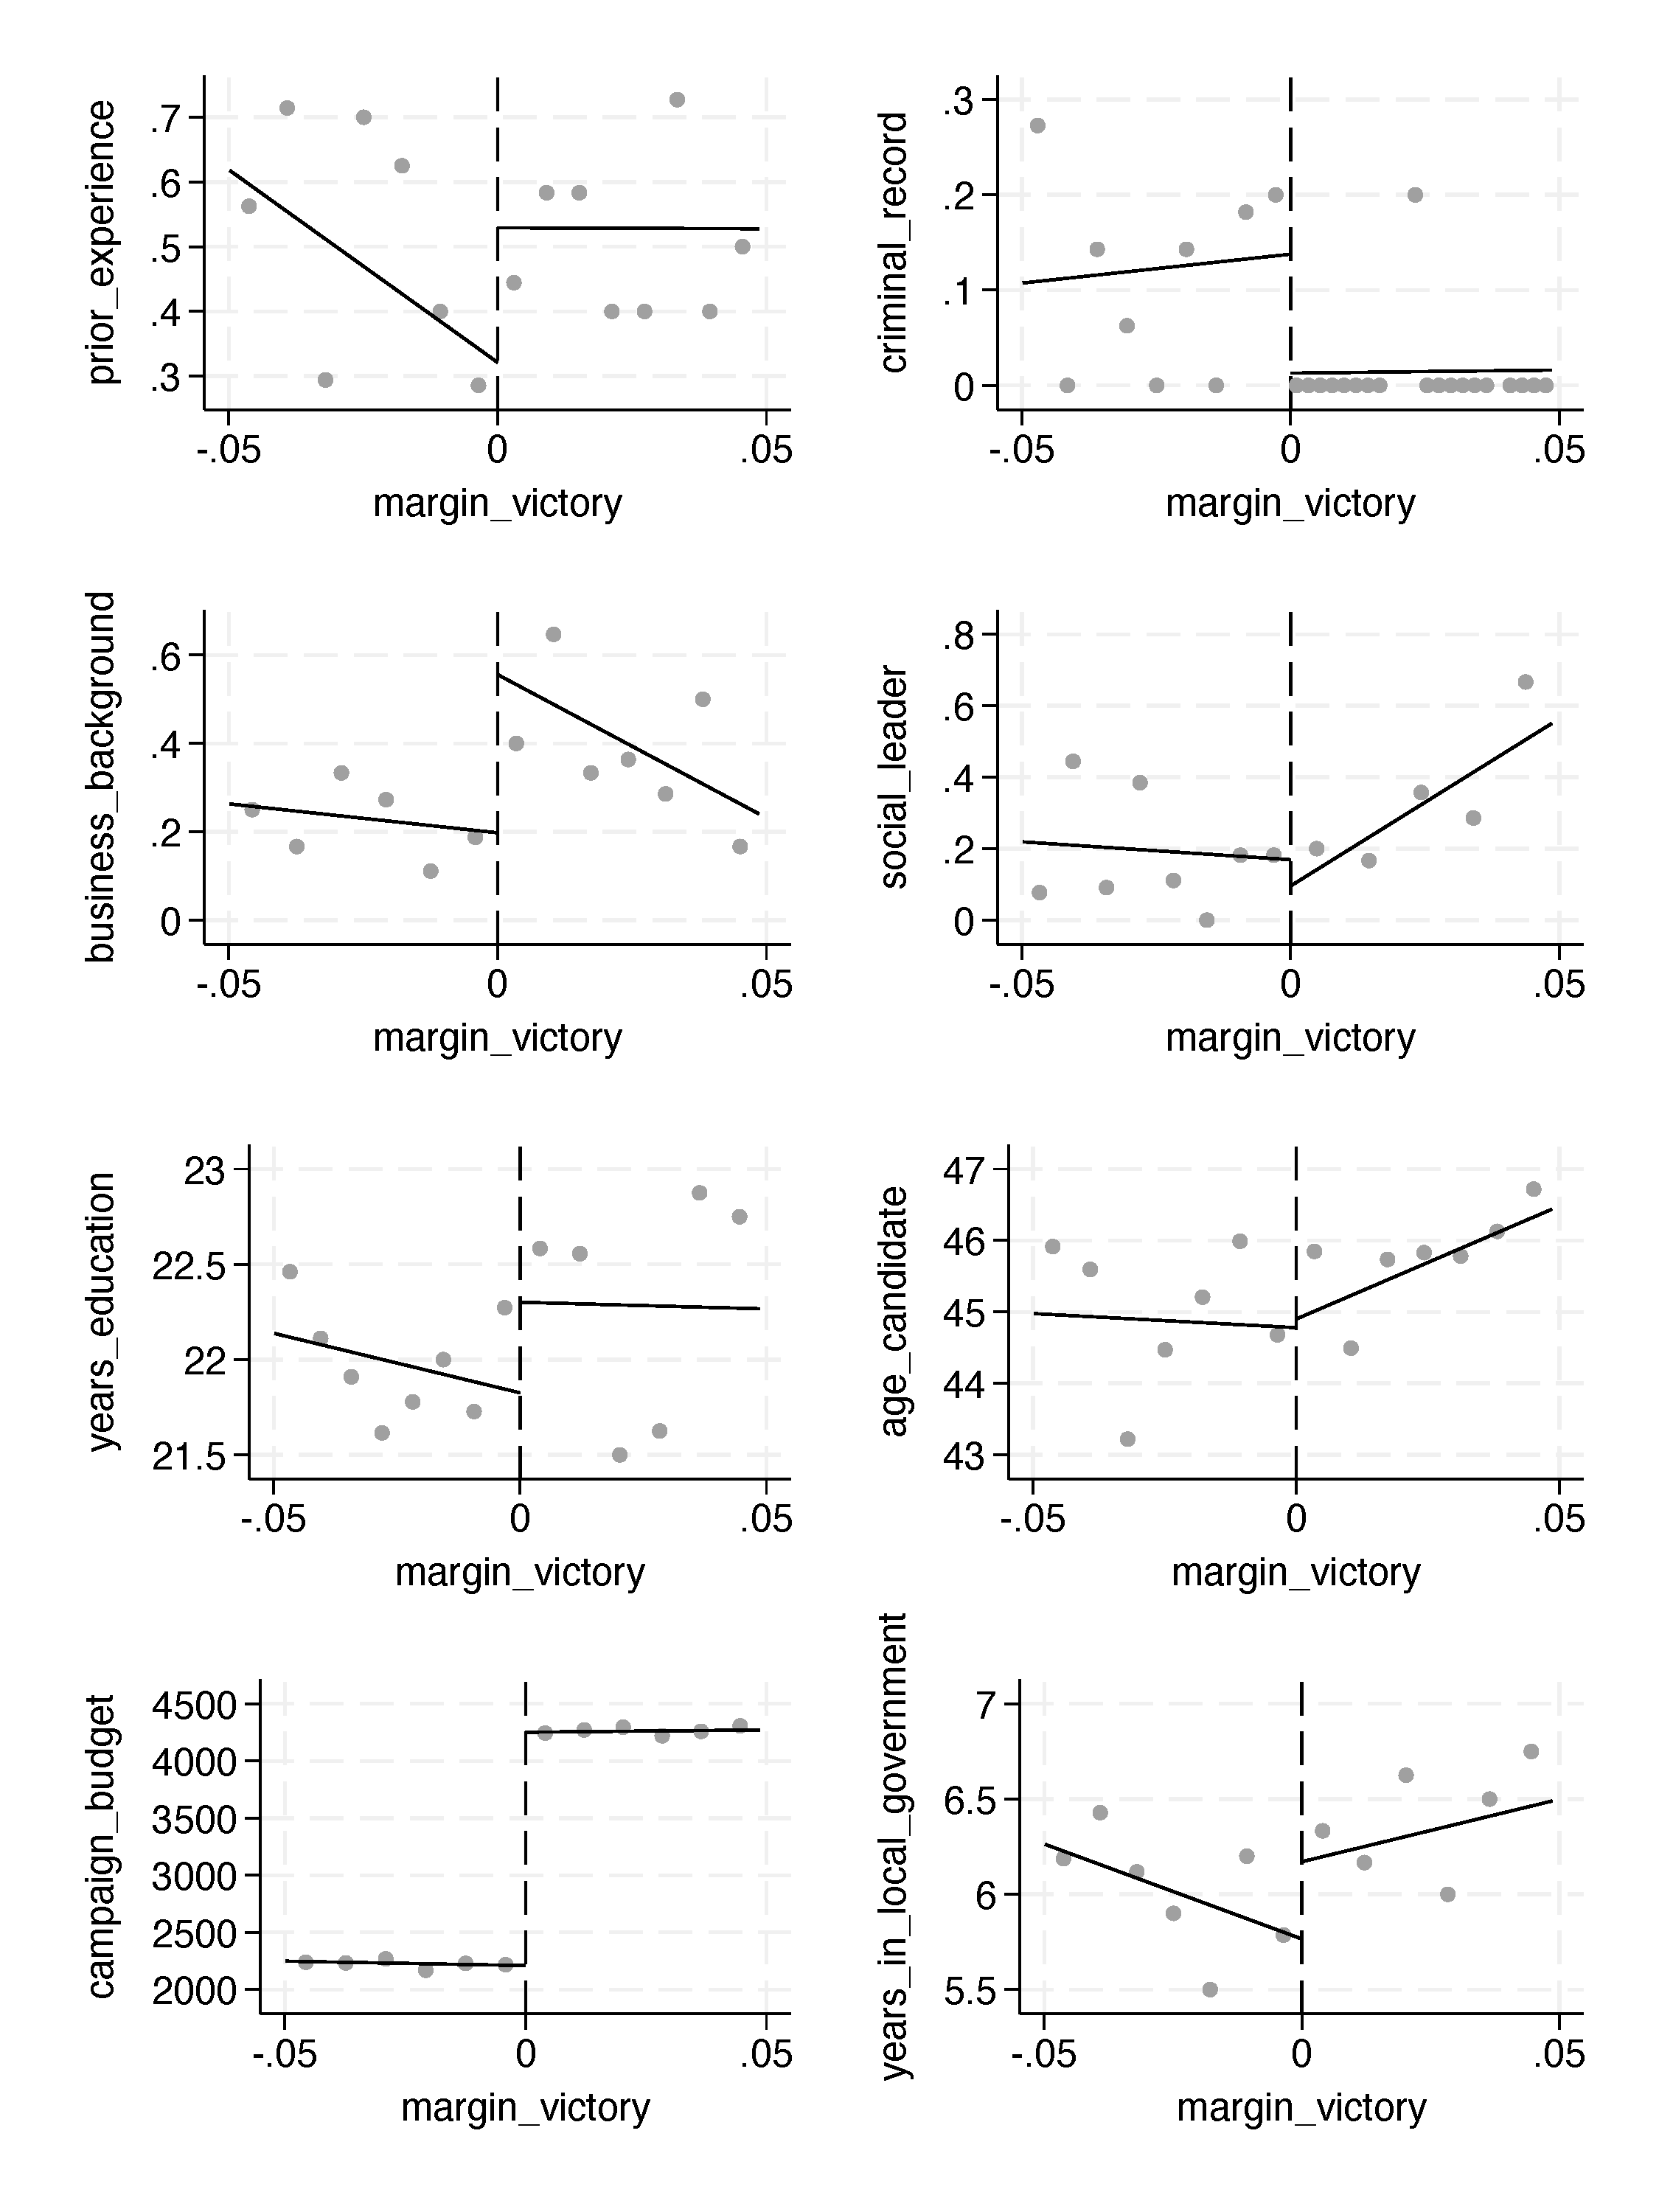
\includegraphics[scale=0.5]{../outputs/characteristics_binned_scatter_esmv_linear_plot.pdf}
    \caption{RDD model robustness}
    \label{fig:characteristics}
\end{figure}

\begin{figure}[H]
    \centering
    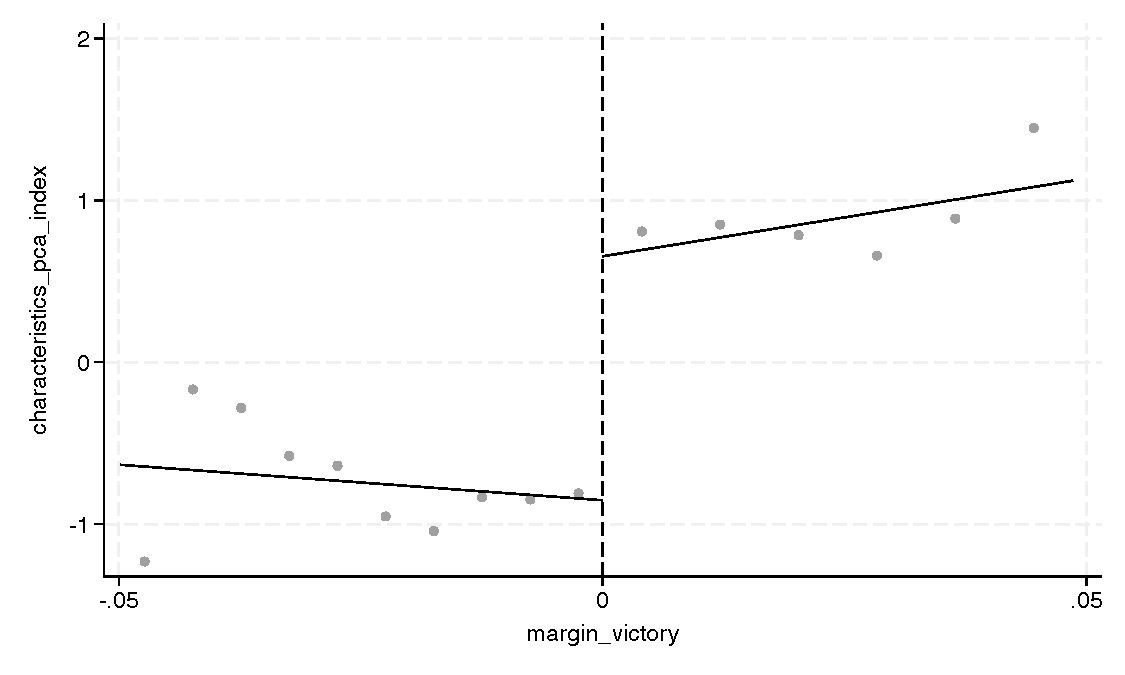
\includegraphics[scale=0.5]{../outputs/characteristics_pca_index_binned_scatter_esmv_linear_plot.pdf}
    \caption{RDD model robustness}
    \label{fig:pca_index}
\end{figure}

\def\sym#1{\ifmmode^{#1}\else\(^{#1}\)\fi}
\begin{adjustbox}{max
width={\textwidth},caption={Candidate characteristic RDD analysis\label{tab:characteristics}},nofloat=table}
\begin{tabular}{l*{9}{c}}
\toprule
                    &\multicolumn{1}{c}{pca\_index}&\multicolumn{1}{c}{prior\_experience}&\multicolumn{1}{c}{criminal\_record}&\multicolumn{1}{c}{business\_background}&\multicolumn{1}{c}{social\_leader}&\multicolumn{1}{c}{years\_education}&\multicolumn{1}{c}{age\_candidate}&\multicolumn{1}{c}{campaign\_budget}&\multicolumn{1}{c}{years\_in\_local\_government}\\
\midrule
RD\_Estimate         &       1.934\sym{**} &       0.179         &      -0.303         &      0.0150         &      0.0274         &       0.525         &       1.629         &      2038.0\sym{***}&       0.673         \\
                    &      (2.84)         &      (0.60)         &     (-1.26)         &      (0.05)         &      (0.11)         &      (0.60)         &      (0.98)         &     (21.42)         &      (0.93)         \\
\midrule
Observations        &         152         &         152         &         152         &         152         &         152         &         152         &         152         &         152         &         152         \\
\bottomrule
\multicolumn{10}{p{\textwidth}}{\centering \footnotesize \textit{t} statistics in parentheses}\\
\multicolumn{10}{p{\textwidth}}{\centering \footnotesize \sym{*} \(p<0.05\), \sym{**} \(p<0.01\), \sym{***} \(p<0.001\)}\\
\end{tabular}\end{adjustbox}


Testing for discontinuities is candidate characteristics, we get the following estimates (see table \ref{tab:characteristics} and figure \ref{fig:characteristics}). I include a principal component analysis index of all the characteristics together (see table \ref{tab:characteristics} and figure \ref{fig:pca_index}). The RDD estimates are strongly significant for campaign budget and principal component analysis index. This implies that compensating differentials affect Dell's results: what we thought was the treatment effect of a PAN victory seems in fact to be the compound treatment effect of a PAN victory and the compensating differential in terms of campaign budget.

Covariate adjustment in a RDD is not sufficient to address the problem of compensating differentials, because these differentials introduce biases that are inherently linked to both observable and unobservable characteristics. Even if observable covariates balanced or controlled for, unobservable characteristics (e.g., competence) could vary discontinuously at the threshold, biasing the treatment effect. Also, covariates may include variables affected by the treatment itself (e.g., campaign funding postulated by voter - donors - and party organization expectations of winning). Including these covariates would introduce post-treatment bias (conditioning on factors influenced by the treatmet), contaminating causal estimates.

All in all, covariate adjustment can reduce noise and account for observable imbalances, but it cannot fully address biases introduced by compensating differentials, especially when unobservable factors are at play.

%%%%%%%%%%%%%%%%%%%%%%%%%%%%%%%%%%%%%%%%%%%%%%%%%%%%%%%%%%%%%%%

\subsection{}

To bound the effect of a PAN mayor on the homicide rate, we implement:
\[
\hat{\tau}^{corr}_{PCRD}
=\hat{\tau}_{PCRD}
-\sum_{k} \hat{\gamma}_k \hat{\delta}_k
\]
With:
\begin{itemize}
    \item index \(i\) for candidates,
    \item index \(d\) for district,
    \item index \(k\) for covariates,
    \item \(\hat{\gamma}_k\) an estimate of the LATE of each compensating differential \(Z_{idk}\),
    \item
    \(
    \delta_k
    =
    E[Z_{idk}\mid \Delta_d = 0, X_{id}=1, X_{jd}=0]
    -
    E[Z_{idk}\mid \Delta_d = 0, X_{id}=0, X_{jd}=1]
    \),
    \item
    \(
    \Delta_d
    =
    V_{id}-V_{0d}
    \),
    \item \( V_{id}\) and \(V_{0d}\) the vote shares of the most popular candidates of types \(X_{id}=1\) and \(X_{id}=1\) respectively,
    \item  \(X_{id}\) a binary characteristic that helps candidate \(i\) win votes.
\end{itemize}

We implement it using the procdedure described and get normally distributed correction terms centered on \(5.26\) and with a sample standard deviation of \(2.66\) (see figure \ref{fig:correction}).
\begin{figure}[H]
    \centering
    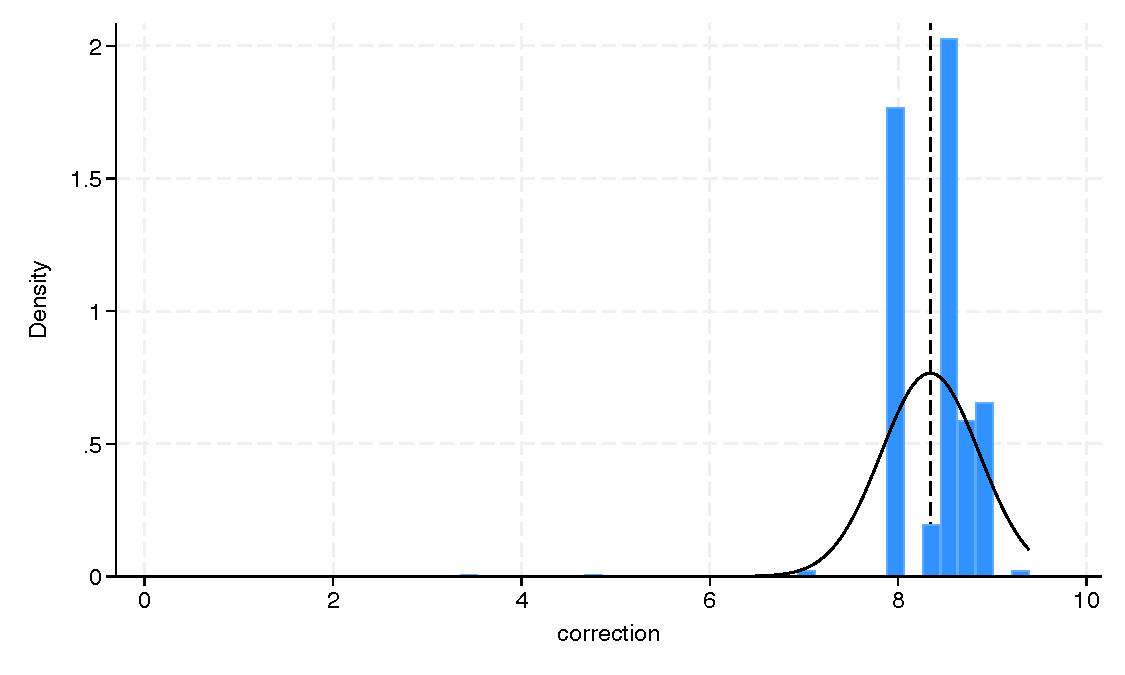
\includegraphics[scale=0.5]{../outputs/correction_term_distribution_plot.pdf}
    \caption{Distribution of the computed correction term}
    \label{fig:correction}
\end{figure}

Recalling that \(\hat{\tau}_{PCRD} = 80.25^{*}\text{ }(2.25)\), the sign and the significance level of our estimate are robust to the (observable) effect of compensating differentials.

\section{}

\subsection{}

We compute the 2SLS estimator and the Wald estimator, as described (see table \ref{tab:IV-2SLS-IV-Wald}). The 2SLS and residualzed Wald estimators are equal.

\begin{table}[htbp]\centering
\def\sym#1{\ifmmode^{#1}\else\(^{#1}\)\fi}
\caption{IV\label{tab:IV-2SLS-IV-Wald}}
\begin{tabular}{l*{2}{c}}
\toprule
                    &\multicolumn{1}{c}{2SLS}&\multicolumn{1}{c}{Wald}\\
\midrule
D                   &       7.633\sym{***}&       7.633\sym{***}\\
                    &     (46.28)         &     (46.02)         \\
\addlinespace
x1                  &       0.124\sym{*}  &                     \\
                    &      (2.25)         &                     \\
\addlinespace
x2                  &      0.0708         &                     \\
                    &      (1.44)         &                     \\
\addlinespace
x1x2                &       0.282\sym{***}&                     \\
                    &      (3.84)         &                     \\
\addlinespace
Constant            &       1.039\sym{***}&       1.208\sym{***}\\
                    &     (10.49)         &     (13.17)         \\
\midrule
Observations        &       10000         &       10000         \\
\bottomrule
\multicolumn{3}{l}{\footnotesize \textit{t} statistics in parentheses}\\
\multicolumn{3}{l}{\footnotesize \sym{*} \(p<0.05\), \sym{**} \(p<0.01\), \sym{***} \(p<0.001\)}\\
\end{tabular}
\end{table}


\subsection{}

A researcher observing \((Y_i,D_i,Z_i,X_i)\) would identify the conditional-on-\(X_i\) LATESs \(E[Y_i(1)-Y_i(0) \mid X_i, G = CP]\) by running 2SLS on the dateset restricted to each level of \(X_i\) respectively. This is an intuition that we can suspect is not relevant considering how unbalanced our data is by construction.

\def\sym#1{\ifmmode^{#1}\else\(^{#1}\)\fi}
\begin{adjustbox}{max
width={\textwidth},caption={Unconditional and conditional LATEs \label{tab:IV-2SLS-IV-Wald-CP}},nofloat=table}
\begin{tabular}{l*{8}{c}}
\toprule
                    &\multicolumn{1}{c}{2SLS X=(0,0)}&\multicolumn{1}{c}{LATE X=(0,0)}&\multicolumn{1}{c}{2SLS X=(1,0)}&\multicolumn{1}{c}{LATE X=(1,0)}&\multicolumn{1}{c}{2SLS X=(0,1)}&\multicolumn{1}{c}{LATE X=(0,1)}&\multicolumn{1}{c}{2SLS X=(1,1)}&\multicolumn{1}{c}{LATE X=(1,1)}\\
\midrule
D                   &       6.680\sym{***}&       5.911\sym{***}&       8.434\sym{***}&       8.126\sym{***}&       6.502\sym{***}&       7.086\sym{***}&       9.139\sym{***}&       9.062\sym{***}\\
                    &     (16.95)         &     (60.13)         &     (37.83)         &     (93.68)         &     (12.48)         &     (73.80)         &     (47.82)         &    (103.33)         \\
\addlinespace
Constant            &       1.587\sym{***}&      0.0624         &       0.828\sym{***}&     -0.0380         &       1.808\sym{***}&     -0.0179         &       0.600\sym{***}&     -0.0129         \\
                    &      (6.97)         &      (0.99)         &      (8.78)         &     (-1.00)         &      (5.70)         &     (-0.24)         &      (5.08)         &     (-0.16)         \\
\midrule
Observations        &        2500         &         417         &        2500         &         833         &        2500         &         417         &        2500         &         833         \\
\bottomrule
\multicolumn{9}{p{\textwidth}}{\centering \footnotesize \textit{t} statistics in parentheses}\\
\multicolumn{9}{p{\textwidth}}{\centering \footnotesize \sym{*} \(p<0.05\), \sym{**} \(p<0.01\), \sym{***} \(p<0.001\)}\\
\end{tabular}\end{adjustbox}


We compute estimated and real coefficients (see table \ref{tab:IV-2SLS-IV-Wald-CP}). As we can see, the 2SLS coefficients are close but upper-biased.

\subsection{}

We compute the convex-weighted average of the conditional LATEs by appropriately using sample means and variances through a series of collapses (see table \ref{tab:Angrist2}). The groups that get the most weight are \(X_i=(1,0)\) and \(X_i=(1,1)\). For the 2SLS estimator to identify the unconditional LATE, we need to have:
\[\forall x \in \{(0,0),(1,0),(0,1),(1,1)\}, E[Y_i(1)-Y_i(0)\mid Xi,G=CP] = E[Y_i(1)-Y_i(0)\mid G=CP] \text{ (constant)}\]
In our data generating process, contrary to what we did, would, \(Y_i(1)\) to be built orthogonal to \(X_i\).

\begin{table}[htbp]\centering
\caption{Weights and convex weighted average of the conditional LATEs\label{tab:Angrist2}}
\begin{tabular}{l*{1}{c}}
\hline\hline
            &\multicolumn{1}{c}{}\\
\hline
Beta 2SLS   &       7.836\\
\hline
Weight00    &       0.542\\
Weight10    &       1.633\\
Weight01    &       0.300\\
Weight11    &       1.525\\
LATEsCvxWghtedAvg&       8.104\\
\hline\hline
\end{tabular}
\end{table}


\subsection{}

If we exclude the \(X_1.X_2\) interaction term from the set of controls, then the estimated effect through \(x_1\) of \(X_i=(1,0)\) is the same as that of \(X_i=(1,1)\). Also, the estimated effect through \(x_2\) of \(X_i=(0,1)\) is the same as the estimated effect of \(X_i=(1,1)\). It is still a convex-weighted average of treatment effects, this time of two treatment effects only.

\subsection{}

\begin{table}[htbp]\centering
\def\sym#1{\ifmmode^{#1}\else\(^{#1}\)\fi}
\caption{Estimated and true unconditional LATEs \label{tab:CPunconditional}}
\begin{tabular}{l*{2}{c}}
\toprule
                    &\multicolumn{1}{c}{2SLS}&\multicolumn{1}{c}{LATE}\\
\midrule
D                   &       8.227\sym{***}&       8.116\sym{***}\\
                    &     (69.70)         &    (158.84)         \\
\addlinespace
Constant            &       0.883\sym{***}&     -0.0122         \\
                    &     (13.39)         &     (-0.34)         \\
\midrule
Observations        &       10000         &        2500         \\
\bottomrule
\multicolumn{3}{l}{\footnotesize \textit{t} statistics in parentheses}\\
\multicolumn{3}{l}{\footnotesize \sym{*} \(p<0.05\), \sym{**} \(p<0.01\), \sym{***} \(p<0.001\)}\\
\end{tabular}
\end{table}


A researcher observing \((Y_i,D_i,Z_i,X_i)\) would identify the unconditional LATES \(E[Y_i(1)-Y_i(0) \mid G = CP]\) by running 2SLS on the dateset without controlling for \(X_i\). This is an intuition that we can suspect is not relevant considering how unbalanced our data is by construction.

We compute estimated and real coefficients (see table \ref{tab:CPunconditional}). As we can see, the 2SLS coefficient is close but upper-biased.


\begin{thebibliography}{9}

\bibitem{dell2015}
Dell, Melissa. “Trafficking Networks and the Mexican Drug War.” American Economic Review 105, no. 6 (2015): 1738-1779.

\bibitem{marshall2024}
Marshall, J. (2024), Can Close Election Regression Discontinuity Designs Identify Effects of Winning Politician Characteristics?. American Journal of Political Science, 68: 494-510.

\bibitem{marshall2024}
Joshua D. Angrist, Guido W. Imbens, 1995. "Average Causal Response with Variable Treatment Intensity," NBER Technical Working Papers 0127, National Bureau of Economic Research, Inc.

\end{thebibliography}

\end{document}